%%% Questions:


\documentclass[12pt,letterpaper]{ntdhw}


\usepackage{ntdmath}
\usepackage{subcaption}
\usepackage{calc}
\usepackage{tikz}
\usepackage{graphicx}
\usetikzlibrary{patterns}

\title{Project 1: PDDL and Constraint-Based Planning}
\author{CSCI 498/598 -- Robot Planning and Manipulation}
\date{Spring 2019}

\rhead{Names:}

%\keytrue

\begin{document}
\pagestyle{fancyplain}

\maketitle
\thispagestyle{fancyplain}
%\clearpage

\begin{enumerate}

  \item Apply your Trivial-SATPlan implementation to the Sussman
  Anomaly in \autoref{fig:sussman}.  What is the resulting plan?

  \item Imagine that you have purchased the new side table (some
  assembly required) in \autoref{fig:lack} only to discover that it
  comes with the ``instructions'' in \autoref{fig:instr}. Construct a
  planning domain to determine the correct assembly steps,
  \begin{enumerate}
    \item Explain the meaning of each predicate in your domain
    \item Explain the meaning of each action in your domain
    \item Attach the PDDL files for you planning domain.
  \end{enumerate}


  \item Download at least one of the following planners and run on
  your PDDL files for question 2.  What are the resulting plans?
  \begin{itemize}
    \item Blackbox:
    \url{https://www.cs.rochester.edu/u/kautz/satplan/blackbox/}
    \item Madagascar:
    \url{http://research.ics.aalto.fi/software/sat/madagascar/}
    \item FF:
    \url{https://fai.cs.uni-saarland.de/hoffmann/ff.html}
  \end{itemize}

  \item Apply your Trivial-SATPlan implementation to your PDDL model
  from question 2.  What is the resulting plans?

  \item The Trivial-SATPlan implementation is (probably) slower than
  the above planners.  What are some reasons for the performance
  difference?

  \item One could correctly claim that ``Constraint-based planning''
  is really just ``heuristic search.''  Why?

  \item To actually execute a plan on a robot arm (physical or
  simulated), we need more than just a symbol such as {\tt pick-up-A}.
  Discuss the additional details or considerations that would be
  necessary to extend your planning domain from question 2 for a robot
  arm.

\end{enumerate}



\tikzstyle{A} = [fill=red!10!white]
\tikzstyle{B} = [fill=green!10!white]
\tikzstyle{C} = [fill=blue!10!white]
\tikzstyle{block} = [rectangle, color=black, draw=black,minimum
height=1.5em, minimum width=1.5em, node distance=1.5em]

\newcommand{\nvar}[2]{%
    \newlength{#1}
    \setlength{#1}{#2}
}
\nvar{\dg}{1.5em}
\def\grip{%
  \node[coordinate] at (.5\dg,0) (gripper) {};
  \draw[double distance=.5em, very thick] (0,0) -- ++(-1em,0);
  \draw[ultra thick](0cm,\dg)--(0cm,-\dg);
  \fill (0cm, 0.5\dg)+(0cm,3.0pt) -- +(1\dg,0cm) -- +(0pt,0pt);
  \fill (0cm, -0.5\dg)+(0cm,0pt) -- +(1\dg,0cm) -- +(0pt,-3pt);
}
\newcommand{\fbdground}[2] {%
  \draw (-#1/2,0)-- (#1/2,0); % line
  \fill[pattern=north east lines,name=ground] (-#1/2,0) rectangle (#1/2,-#2); % hashes
}


\begin{figure}
  \begin{minipage}{.55\textwidth}
    \subcaptionbox{}{
      \begin{small}
        \listpddl{pddl/blocksworld/blocks-domain.pddl}
      \end{small}
    }
  \end{minipage}
  \begin{minipage}{.40\textwidth}
    \subcaptionbox{}{
      \begin{tikzpicture}[node
        distance=2em,title/.style={font=\Large\bf}]
        \fbdground{6em}{.75em}
        \node[block,B,name=B,xshift=-1.5em, yshift=.75em] {B};
        \node[block,A,name=A, right of=B, xshift=1.5em] {A};
        \node[block,C,name=C, above of=A] {C};
        \node[font=\Large\bf,yshift=6em] {Start};
        \begin{scope}[xshift=10em]
          \fbdground{6em}{.75em}
          \node[block,A,name=A, yshift=.75em] {A};
          \node[block,B,name=B, above of=A] {B};
          \node[block,C,name=C, above of=B] {C};
          \node[title,yshift=6em] {Goal};
        \end{scope}
      \end{tikzpicture}
    }

    \vspace{12em}

    \subcaptionbox{}{
      \listpddl{pddl/blocksworld/sussman-anomaly.pddl}
    }
  \end{minipage}
  \caption{Blocksworld planning domain and Sussman Anomaly Example}
  \label{fig:sussman}
\end{figure}

%\def\scal{1.35}
\begin{figure}
  \begin{subfigure}{.5\textwidth}
    \centering
    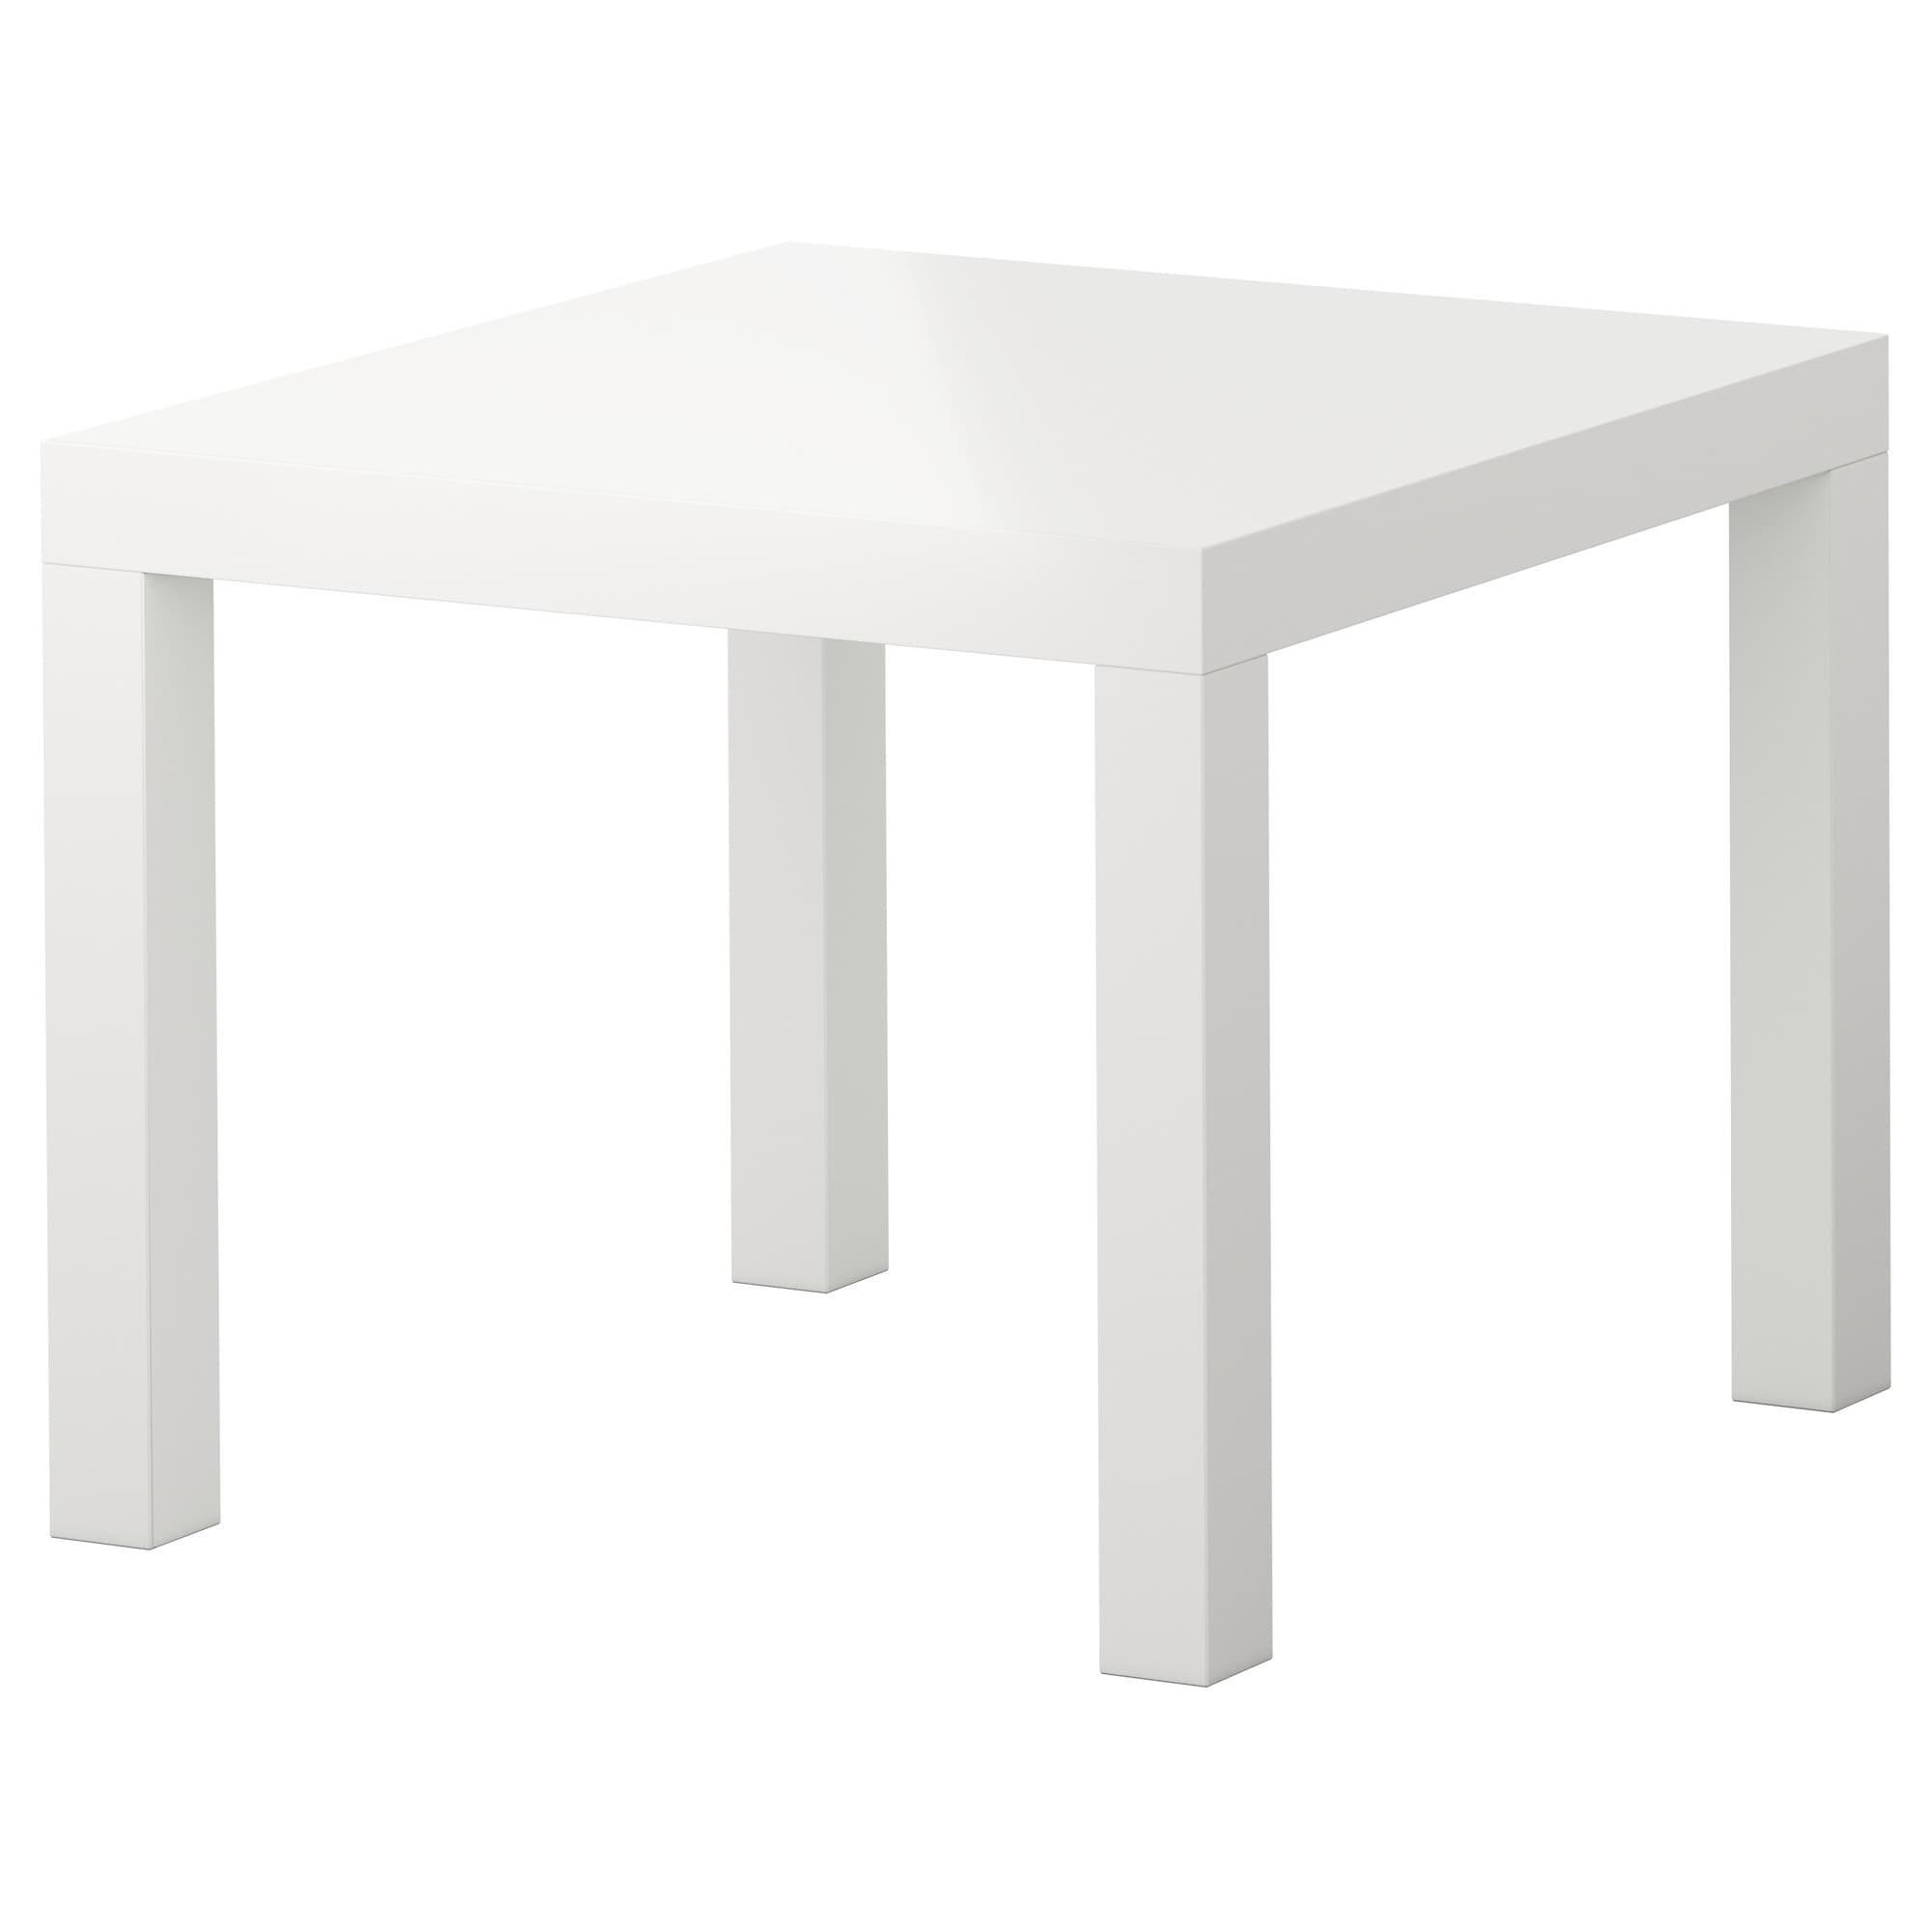
\includegraphics[height=22em]{ikea/lack.jpg}
    \caption{}
    \label{fig:lack}
  \end{subfigure}
  \hfil
  \begin{subfigure}{.5\textwidth}
    \centering
    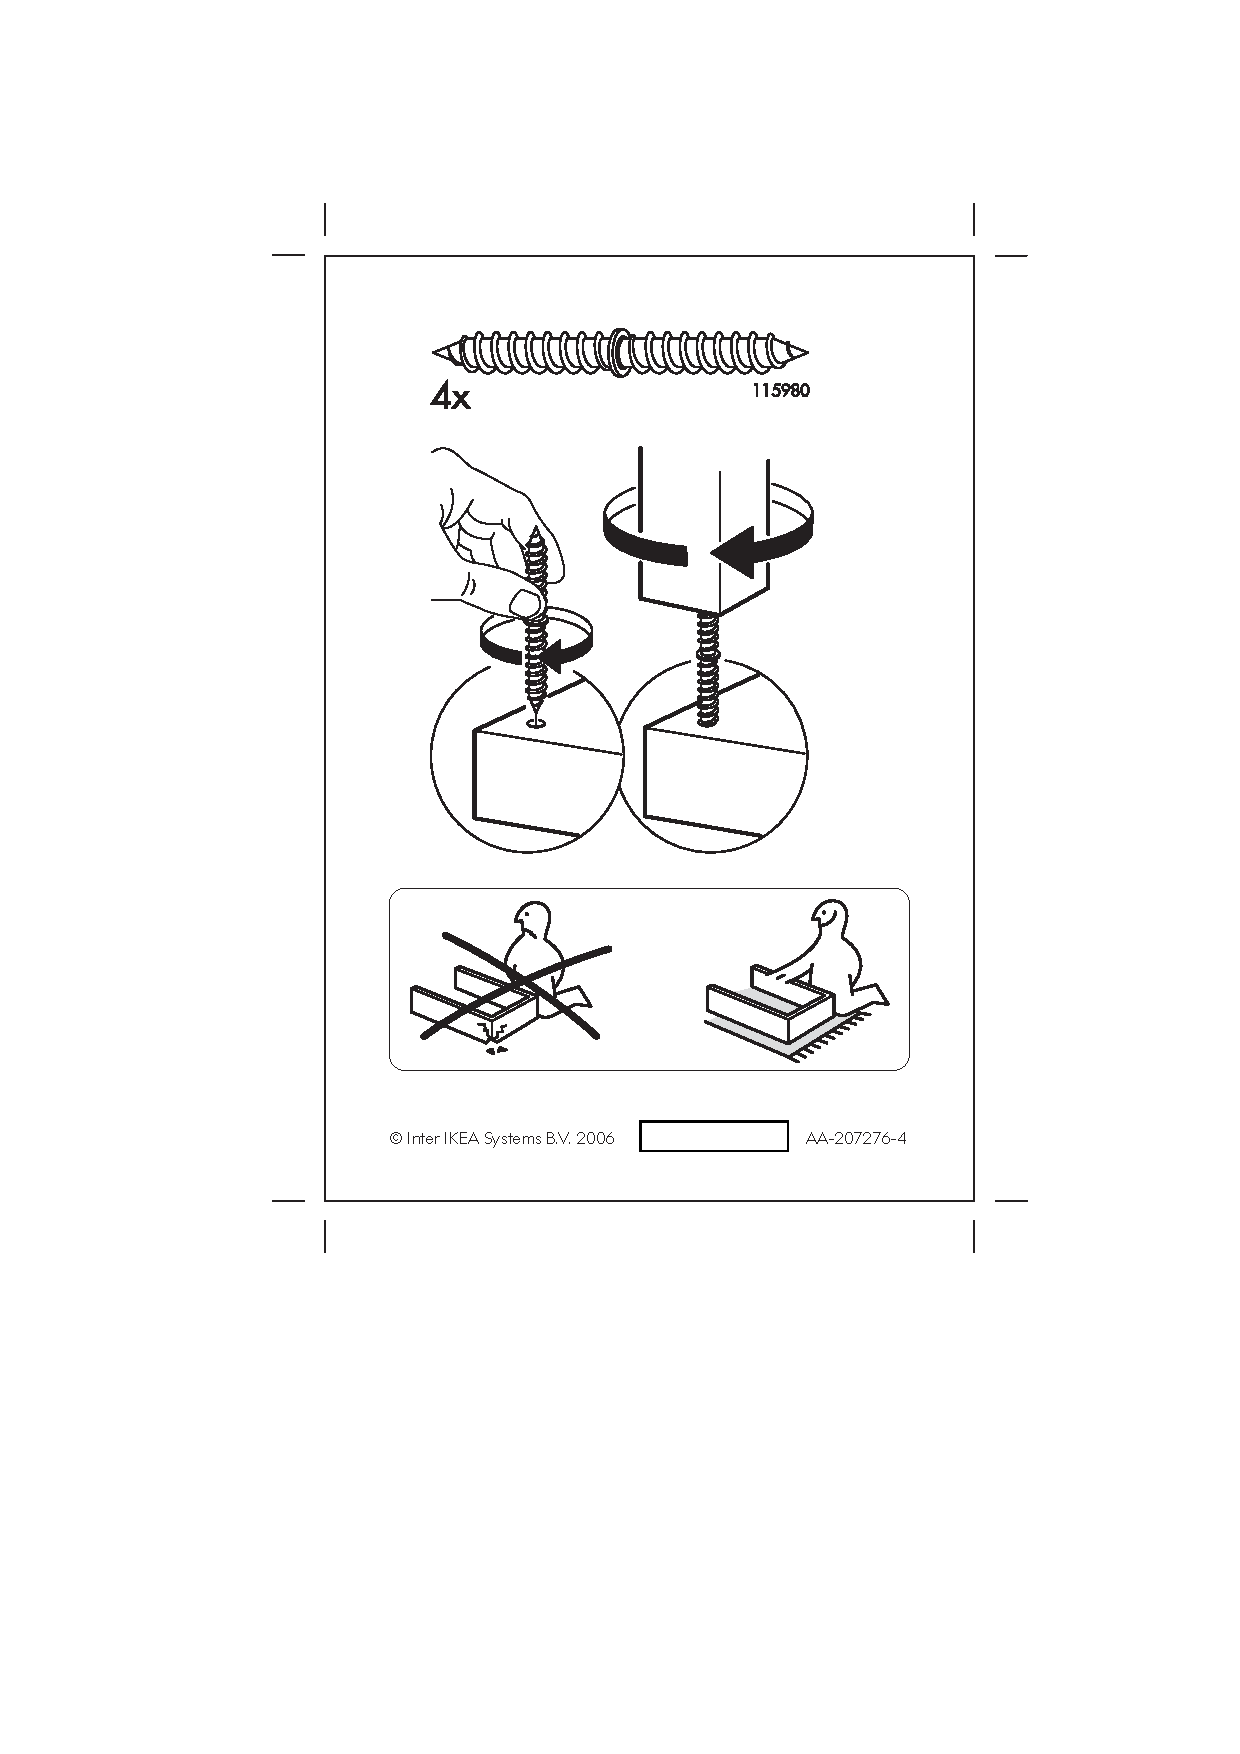
\includegraphics[height=22em,clip,trim={2.25in 4in 2.25in 2in}]{ikea/lack-instr.pdf}
    \caption{}
    \label{fig:instr}
  \end{subfigure}
  % \subcaptionbox{}{
  %   \includegraphics[height=8em*\real{\scal}]{sokoban/sokoban-2.png}
  % }\hfil
  % \subcaptionbox{}{
  %   \includegraphics[height=8em*\real{\scal}]{sokoban/sokoban-3.png}
  % }
  \caption{Ikea ``Lack'' side table}
  \label{fig:sokoban}
\end{figure}

\end{document}

%%% Local Variables:
%%% mode: latex
%%% TeX-master: t
%%% End:
